\subsection{Mô hình hỗn hợp trong môi trường đa nhiệm}
Trong thống kê mô hình hỗn hợp (thuật ngữ gốc: \emph{mixture models}) là mô hình xác suất đại diện cho sự hiện diện của các quần thể con trong tổng thể \cite{rasmussen2000infinite}. Nói cách khác mô hình hỗn hợp là một hỗn hợp các phân phối xác suất đại diện cho các tập hợp con tạo thành quần thể.
\\[0.5cm]
\begin{figure}[h!]
    \centering
        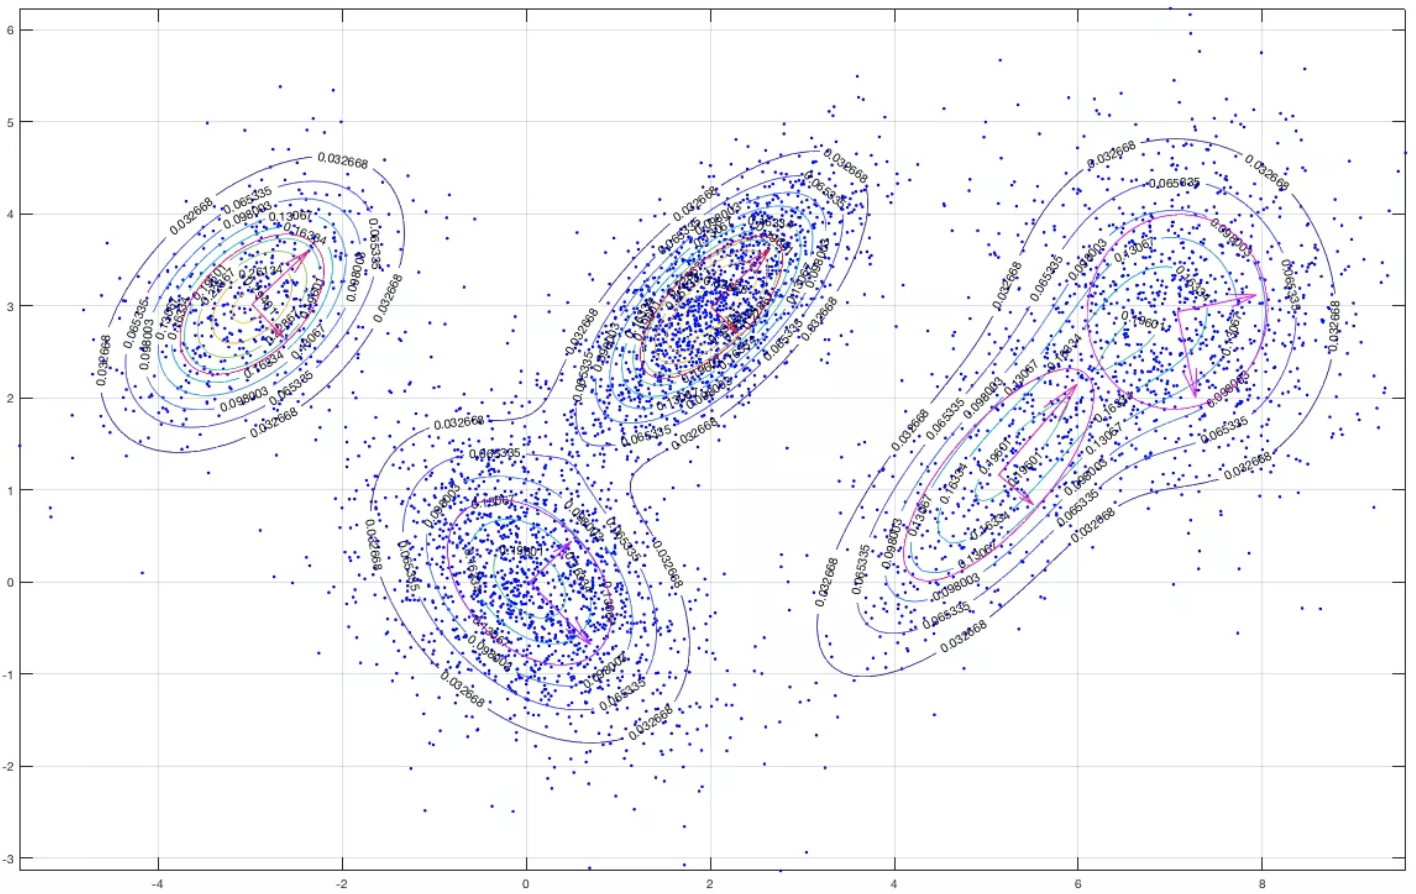
\includegraphics[width=9cm]{mixture-model.png}
    \caption{Ví dụ về mô hình hỗn hợp trong quần thể}
    \label{fig:mixture-model}
\end{figure}

Không làm mất tính tổng quát, ta coi $P^k$ là tập hợp các quần thể con liên kết với tác vụ thứ $k$ trong tập các tác vụ $k \in \{1,2,...K\}$. Hàm mục tiêu là $f_k$ và $f_k^* = f_k(x^*)$ là cực đại toàn cục tại tác vụ thứ $k$. Trong tiến hóa đa nhiệm, mỗi tác vụ các tác vụ tại một thế hệ thứ $t > 0$ có tập các quần thể con tương ứng với phân xác suất là $p^1(x,t), p^2(x,t),...., p^k(x,t)$. Sự tương tác giữa các tác vụ, quần thể con cái được sinh ra tại thế hệ thứ $t$ và bởi tác vụ thứ $k$ được biểu diễn dưới dạng một mô hình hỗn hợp như sau:
\begin{equation}
    q^k(x,t) = \alpha_k \cdot p^k(x,t) + \sum_{j \neq k} \alpha_j \cdot p^j(x,t)
    \label{equa:mixture_distribution}
\end{equation}
Ở đây phân phối $q^k(x,t)$ là một hỗn hợp $K$ phân phối với hệ số hỗn hợp là $\alpha^{'}s$. Có $\alpha_k + \sum_{j \neq k} \alpha_j = 1$ và $\alpha^{'}s >= 0$. 

Có thể thấy việc chia sẻ tri thức trong môi trường đa nhiệm là hệ quả của quá trình lấy mẫu các giải pháp phù hợp từ những phân phối hỗn hợp trong công thức \ref{equa:mixture_distribution}. Tuy nhiên trong trường hợp thiếu đi những tri thức tiên nghiệm về mối quan hệ giữa các tác vụ, việc chia sẻ tri thức có nguy cơ cao không những tri thức được chia sẻ không giúp các tác vụ tối ưu hóa nhanh hơn mà còn khiến nó bị giảm tốc độ. Hay nói cách khác là chia sẻ âm (thuật ngữ gốc: \emph{negative transfer}). Vậy vấn đề cần đặt ra là làm thế nào để xác định khi nào cần chia sẻ tri thức, khi nào không và mức độ chia sẻ là bao nhiêu. Điều này được thể hiện ở hệ số hỗn hợp $\alpha^{'}s$, giá trị $\alpha^{'}s$, và các hệ số này cần được học và tối ưu tại mỗi thế hệ sao cho phù hợp nhất với mối quan hệ giữa các tác vụ tại thời điểm đang xét.

Vậy thuật toán MFEA-I đã mô tả ở (\ref{mfeai}) với điểm nổi bật là khả năng chia sẻ tri thức giữa các tác vụ tối ưu khác nhau có gặp vấn đề negative transfer không? Dưới đây tôi sẽ đi vào phân tích thuật toán MFEA-I dưới một góc độ khác, góc độ xác suất để để trả lời cho câu hỏi đó.

\subsection{Phân tích tiến hóa đa nhiệm dưới góc độ xác suất}
Để dễ dàng phân tích thuật toán MFEA-I dưới góc độ xác suất thì không mất tính tổng quát, đưa ra một số giả thiết sau:
\begin{itemize}
    \item Toán tử sinh sản trong thuật toán MFEA-I tuân theo quy tắc xoay quanh cha mẹ (thuật ngữ gốc: \emph{parent-centric}), có nghĩa quần thể con được sinh ra có xác suất cao nằm gần với bố mẹ. 
    % Thực tế việc giả định này nhằm đơn giản việc phân tích, thay vì \emph{parent-centric} thì toán tử sinh sản ngẫu nhiên cũng sẽ có kết quả tương tự, tôi sẽ để phần chứng minh tại phụ lục bổ sung. 
    \item Phân phối xác suất của quần thể cha mẹ tuân theo phân phối chuẩn nhiều chiều.
    % với trung vị là $m$ và hiệp phương sai là $\sum$. Điều này dẫn đến hệ quả là phân phối của tập con cái sẽ rất gần với phân phối của tập cha mẹ: $p_c(x,t) \approx p(x,t)$. 
\end{itemize}
Giống như phần mô tả \emph{mô hình hỗn hợp trong môi trường đa nhiệm} ở trên, trong MFEA-I ta có thể định nghĩa lại như sau:
\begin{itemize}
    \item Tại thế hệ thứ $t$, cả $K$ tác vụ sẽ có quần thể chung là $P_t$
    \item Tại thế hệ thứ $t$ mỗi tác vụ thứ $k$ có tập quần thể con liên kết với nó là $P_t^k$
    \item $P_t$ được biểu diễn bởi mô hình $p(x,t)$, con cái của chúng được biểu diễn bởi $p_c(x,t)$
    \item $P_t^k$ được biểu diễn bởi mô hình $p^k(x,t)$, con cái của chúng được biểu diễn bởi $p_c^k(x,t)$
\end{itemize}
Tuân theo giả thiết về toán tử parent-centric, một ước lượng toàn bộ quần thể $p_c(x,t) \approx p(x,t)$. Tuy nhiên những cá thể con cái thuộc tác vụ $k$ được sinh ra do quá trình trao đổi chéo của bố mẹ là $p_c^k(x,t)$ thì \textbf{không nhất thiết phải tuân theo nguyên tắc này}.
Ta có mô hình hỗn hợp phân phối của tập con cái tại thế hệ thứ $t$ của tác vụ $k$ được biểu diễn bởi:
\begin{equation}
    p_c^k(x,t) = [1 - \frac{0.5 \cdot (K - 1) \cdot rmp}{K} ] \cdot p^k(x,t) + \sum_{j \neq k}\frac{0.5 \cdot rmp}{K} \cdot p^j(x,t).
    \label{equa:mfea_offstring_distribution}
\end{equation}
Trong đó các hệ số $\alpha_k$ và $\alpha_j$ của công thức \ref{equa:mixture_distribution} được thay thế lần lượt bởi $[1 - \frac{0.5 \cdot (K - 1) \cdot rmp}{K} ] $ và $\frac{0.5 \cdot rmp}{K}$. 
% Phần chứng minh các hệ số này tôi xin phép đặt tại phụ lục bổ sung. \emph{Phải chứng minh cái này}

Theo công thức \ref{equa:mfea_offstring_distribution}, có thể thấy hệ số hỗn hợp $\alpha$ phụ thuộc vào giá trị $rmp$. Tuy nhiên trong thuật toán MFEA-I thì hệ số $rmp$ là cố định dùng chung cho tất cả các cặp tác vụ được chọn ngay từ khi khởi tạo. Hệ số này càng lớn thì khả năng chia sẻ, khả năng trao đổi chéo khác tác vụ càng lớn  hoặc ngược lại khi hệ số này càng nhỏ thì việc chia sẻ, trao đổi tri thức gần như không xảy ra. Hay nói cách khác thuật toán MFEA-I sẽ trở về tương tự thuật toán đơn nhiệm thông thường mà không khai thác được mối quan hệ giữa các tác vụ. Tuy nhiên trong trường hợp cặp tác vụ không có sự bổ trợ lẫn nhau thì việc trao đổi là không cần thiết và còn khiến các tác vụ hội tụ chậm hơn so với thuật toán tiến hóa đơn nhiệm thông thường theo chứng minh của Bali, Ong, Gupta and Tan (dẫn chứng).
Với nguyên tắc này phân phối các cá thể mới của tác vụ được sinh ra $p_c^k(x,t)$ như trong công thức \ref{equa:mfea_offstring_distribution} sẽ cần phải càng gần với phân phối của cá thể cha mẹ $p^k(x,t)$ càng tốt (do đã quy định toán từ sinh sản là parent-centric). Hay nói cách khác hệ số hỗn hợp $\alpha_k >> \alpha_j$.
Nhìn vào công thức \ref{equa:mfea_offstring_distribution} thì để thực hiện điều này sẽ có 2 cách:
\begin{itemize}
    \item $rmp = 0$ : Nghĩa là không có sự trao đổi nào giữa các tác vụ, quần thể con cái sinh ra sẽ tuân theo quy luật parent-centric và phân phối của quần thể con cái sẽ gần với quần thể cha mẹ.
    \item $rmp > 0$ : Điều khiển hệ số $rmp$ để xác định và giảm tác động của việc trao đổi âm giữa các tác vụ.
\end{itemize}
Cách thứ nhất thực tế rất đơn giản vì chỉ cần xét $rmp = 0$ tuy nhiên cách này sẽ khiến ta không khai thác được khả năng của tiến hóa đa nhiệm, điểm tốt giữa sự trao đổi tri thức khác tác vụ. Vậy nên phần dưới đây tôi chỉ tập trung vào phương pháp thứ 2 là điều khiển giá trị của $rmp > 0$ để giảm tác động của việc trao đổi âm giữa các tác vụ.

Tuy nhiên, làm thế nào để ước lượng giá trị $rmp$ của từng cặp tác vụ tại từng thời thế hệ sao cho phù hợp với mối quan hệ giữa cặp tác vụ đó để ta đạt được hiệu quả trao đổi tri thức cao nhất? 

Đây cũng là ý tưởng chính mở ra hướng đi mới cho tiến hóa đa nhiệm - thuật toán tiến hóa đa nhiệm với ước lượng hệ số trao đổi $rmp$ trực tuyến, và đây cũng là hướng đi chính cho các giải thuật đề xuất trong đồ án này.
